\documentclass{article}
\usepackage{tikz-qtree}
\begin{document}
\tikzset{every tree node/.style={minimum width=2em,draw,circle},
	    blank/.style={draw=none},
	    edge from parent/.style=
	    {draw,edge from parent path={(\tikzparentnode) -- (\tikzchildnode)}},
	    level distance=1.5cm}
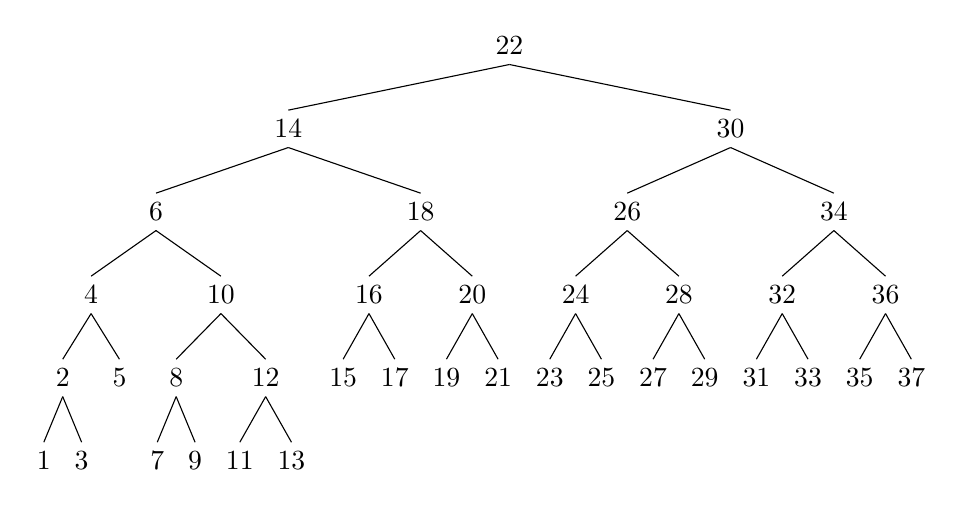
\begin{tikzpicture}
\Tree
[.22
[.14
[.6
[.4
[.2
{1}
{3}
]
{5}
]
[.10
[.8
{7}
{9}
]
[.12
{11}
{13}
]
]
]
[.18
[.16
{15}
{17}
]
[.20
{19}
{21}
]
]
]
[.30
[.26
[.24
{23}
{25}
]
[.28
{27}
{29}
]
]
[.34
[.32
{31}
{33}
]
[.36
{35}
{37}
]
]
]
]
\end{tikzpicture}
\end{document}
